\documentclass{article}
\usepackage{tikz}

\begin{document}

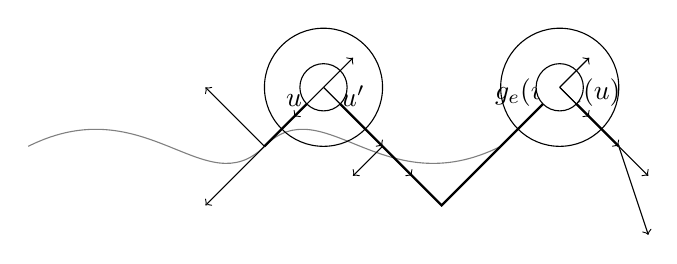
\begin{tikzpicture}[scale=1.5]
    % Draw the original walk in gray
    \draw[gray] (0,0) .. controls (0.5,0.5) and (1,-0.5) .. (2,0);
    \draw[gray] (0,0) .. controls (-0.5,-0.5) and (-1,0.5) .. (-2,0);
    
    % Draw the modified walk in black
    \draw[thick] (0,0) -- (0.5,0.5) node[midway,above] {$u$};
    \draw[thick] (0.5,0.5) -- (1,0) node[midway,above] {$u'$};
    \draw[thick] (1,0) -- (1.5,-0.5) -- (2,0);
    \draw[thick] (2,0) -- (2.5,0.5) node[midway,above] {$g_e(u')$};
    \draw[thick] (2.5,0.5) -- (3,0) node[midway,above] {$g_e(u)$};
    
    % Draw circles around the points u' and g_e(u')
    \draw[fill=white] (0.5,0.5) circle (0.2);
    \draw[fill=white] (2.5,0.5) circle (0.2);
    
    % Draw the circles around the points u' and g_e(u')
    \draw (0.5,0.5) circle (0.5);
    \draw (2.5,0.5) circle (0.5);
    
    % Draw the lines indicating the reflection and extension
    \draw[->] (0.5,0.5) -- (0.75,0.75);
    \draw[->] (2.5,0.5) -- (2.75,0.75);
    
    % Draw the lines indicating the splitting point
    \draw[->] (0.5,0.5) -- (0.25,0.25);
    \draw[->] (2.5,0.5) -- (2.75,0.25);
    
    % Draw the lines indicating the original walk
    \draw[->] (0,0) -- (-0.5,-0.5);
    \draw[->] (0,0) -- (-0.5,0.5);
    
    % Draw the lines indicating the modified walk
    \draw[->] (0.5,0.5) -- (1,0);
    \draw[->] (2.5,0.5) -- (3,0);
    
    % Draw the lines indicating the reflection and extension
    \draw[->] (1,0) -- (1.25,-0.25);
    \draw[->] (3,0) -- (3.25,-0.25);
    
    % Draw the lines indicating the splitting point
    \draw[->] (1,0) -- (0.75,-0.25);
    \draw[->] (3,0) -- (3.25,-0.75);
\end{tikzpicture}

\end{document}